%!TEX ROOT=main.tex

There are many commercially available solutions for soil moisture sensing. Offers range from generic hobby-grade to professional research-grade sensors of different form-factors and utilizing various methods of measurement. Following is a list of offerings approximately sorted by price and capabilities
\begin{itemize}
    \item TEROS 54 and TEROS 10 from METER Group \cite{meter_group_teros_2024, meter_group_teros_nodate}
    \item BL-5311 biSensor by Baseline \cite{baseline_soil_2021}
    \item Generic capacitive soil-moisture sensor available from various sources \cite{czechproject_spol_sro_pudni_2024}
\end{itemize}

\begin{figure}
    \centering
    \subfloat[METER TEROS 10]{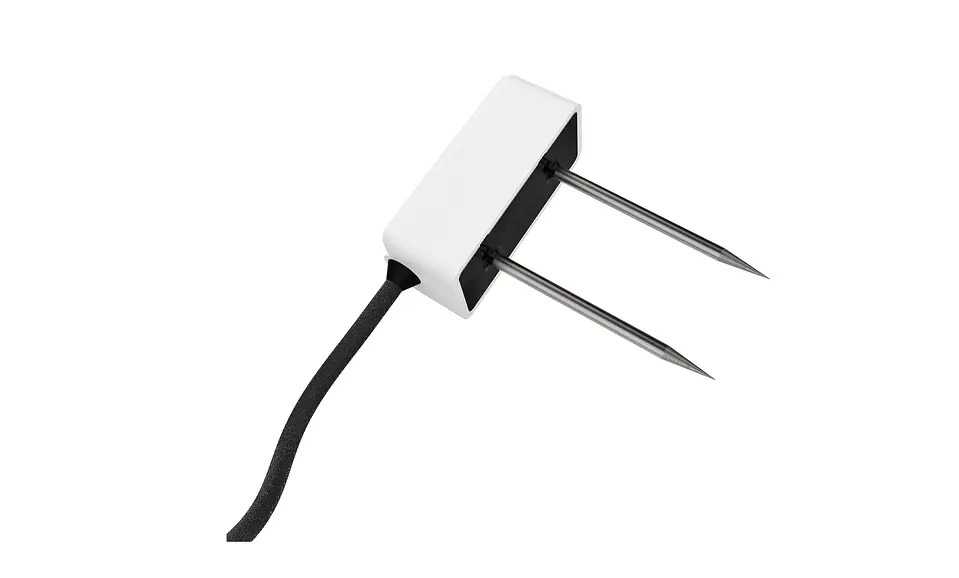
\includegraphics[width=.3\textwidth]{img/sensor-teros10.jpg}}
    \subfloat[Baseline BL-5311]{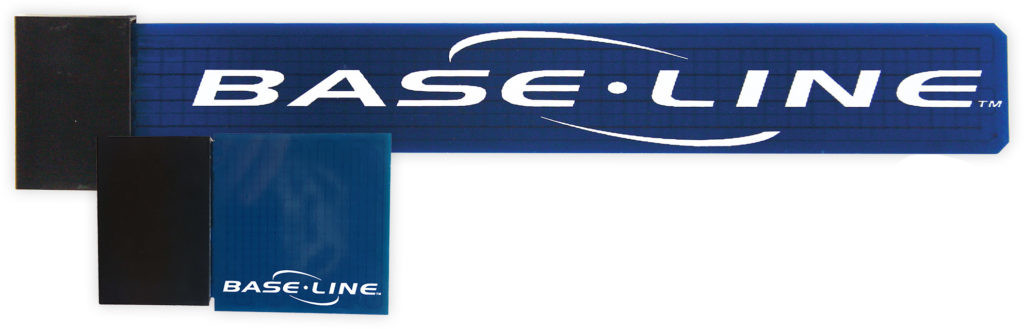
\includegraphics[width=.3\textwidth]{img/sensor-baseline.jpg}}
    \subfloat[Generic sensor]{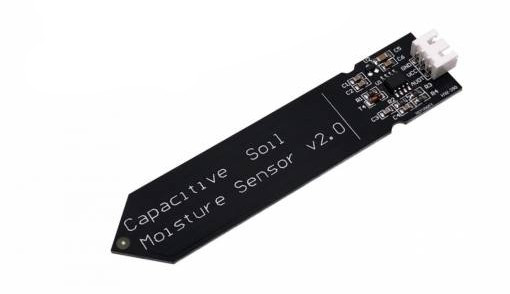
\includegraphics[width=.3\textwidth]{img/sensor-generic.jpg}}
    \caption{\label{fig:soil-sensors}Examples of commercially available soil moisture sensors \cite{meter_group_teros_nodate, baseline_soil_2021, czechproject_spol_sro_pudni_2024}.}
\end{figure}

The Baseline BL-5311 is constructed from an FR4 material and a plastic box housing the electronics. It is designed to be buried 10's of centimeters below the surface near the root zone. The sensor measures volumetric water content using Time Domain Transmissometry (TDT), thus the sensor is galvanically isolated from the soil.

\section{Soil water content}
Soil is made up of a solid phase of minerals and organic matter, and the pours in-between the solids, which hold gasses and water \cite{paul_soil_2007}. The total amount of moisture is the sum of the moisture contained inside the solids (in intra-aggregate pore space) and the space around the solids (inter-aggregate pore space) \cite{myjove_corporation_determination_2024}. This work will not distinguish between the two for simplicity.

\subsection{Definition}
Soil water or moisture content is a ratio, which ranges from 0, meaning completely dry, to the value of material porosity at saturation \cite{webster_humidity_1998}. It expresses the quantity of water contained in the soil. We can measure it by mass (gravimetric method) or by volume, as depicted in Figure \ref{fig:soil-phase-diagram}.

Volumetric content (VWC) can be expressed mathematically as
\begin{equation}
    \label{equation:volumetric-content} \theta = \dfrac{V_w}{V_s + V_w + V_a}
\end{equation}
where $V_w$ is the volume of water and $V_s + V_w + V_a$ is the total volume of the soil sample including contained air. 

Likewise, gravimetric water content (GWC) is defined as
\begin{equation}
    \label{equation:gravimetric-content} u = \dfrac{m_w}{m_s}
\end{equation}
where $m_w$ is the mass of the water and $m_s$ is mass of all solids in the sample \cite{edaphic_scientific_pty_ltd_how_2024}.

\begin{figure}
    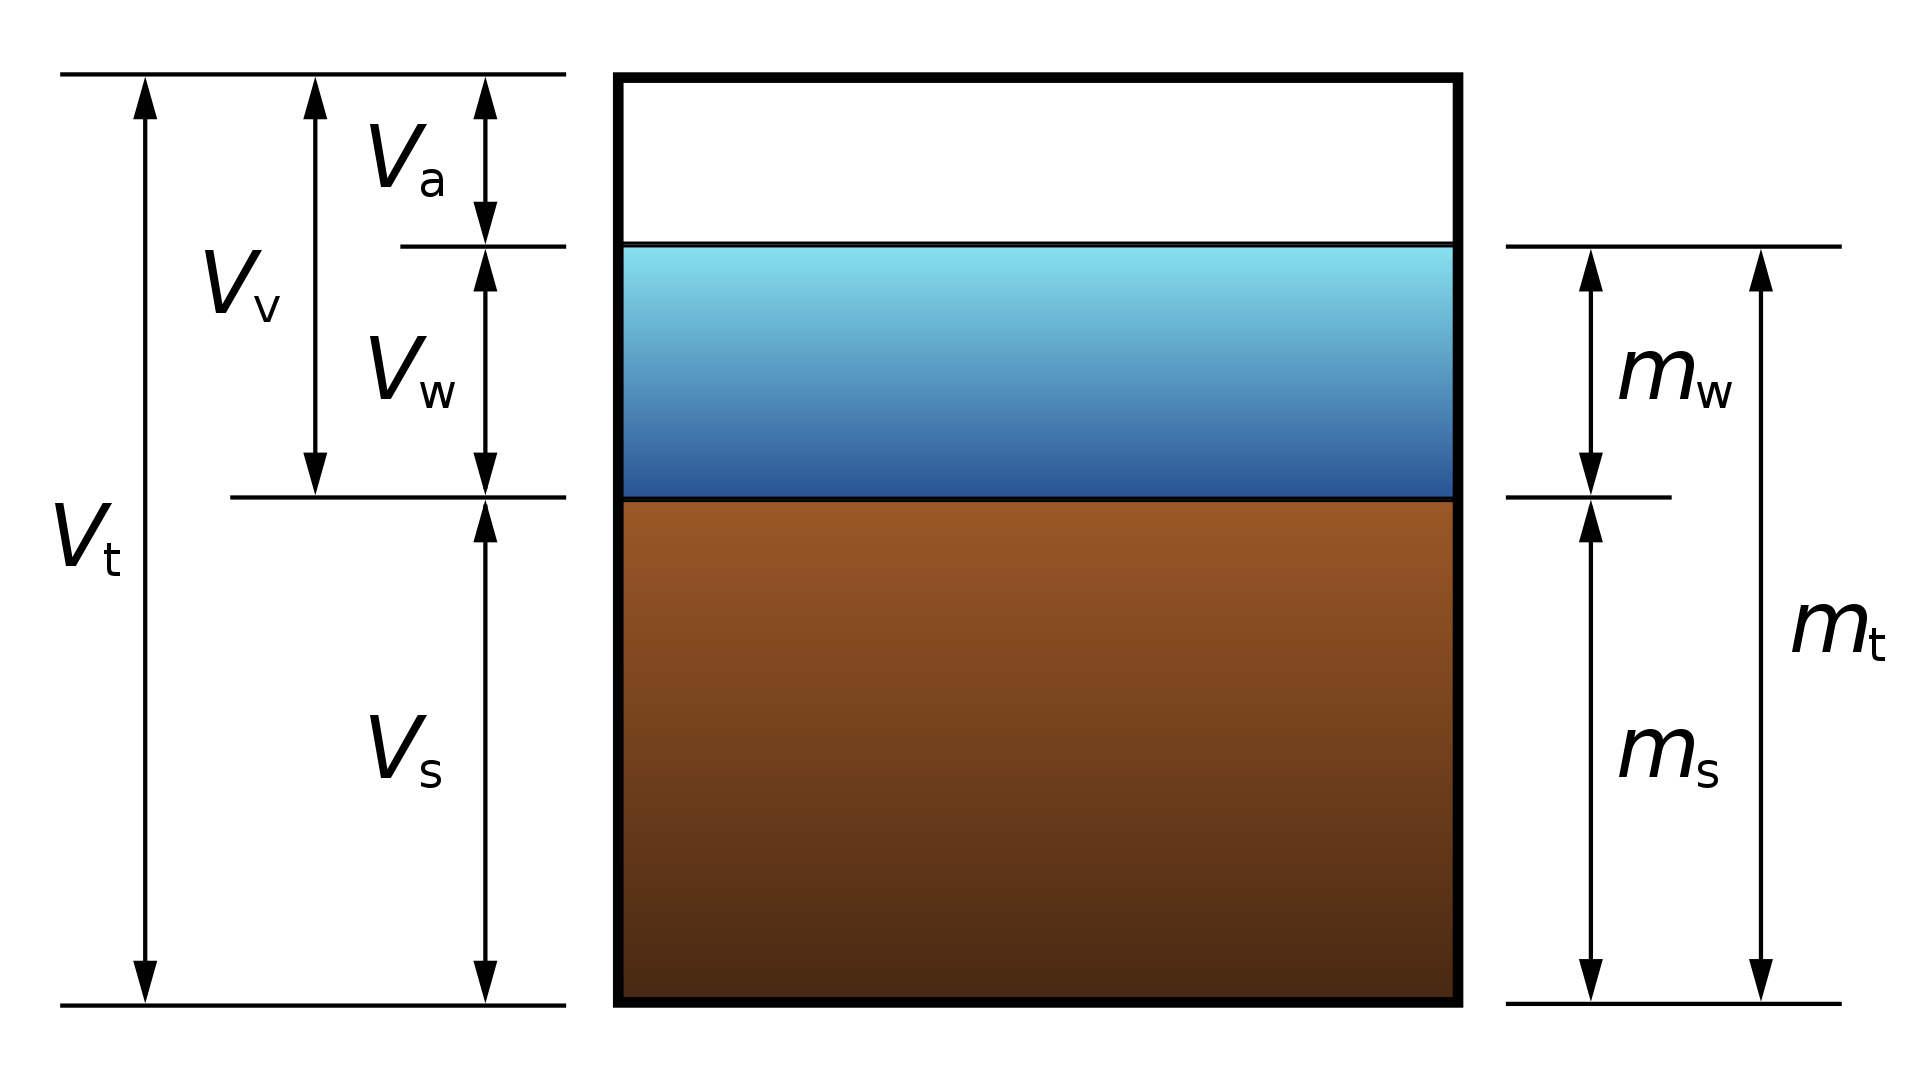
\includegraphics[width=.5\textwidth]{fig/soil-phase-diagram.png}
    \caption{\label{fig:soil-phase-diagram} Soil composition by volume and mass \cite{noauthor_water_2023}.}
\end{figure}

\subsection{Methods of measurement}
\subsubsection{Drying the soil}
Drying the soil sample in a drying oven is a direct method of measurement and is used as the reference method \cite{webster_humidity_1998}. By weighing the sample and also measuring its volume, then doing that again after drying, it is possible to very accurately measure both the volumetric and the gravimetric water content both at the same time.

The procedure involves gathering a known quantity of the sample, ranging from 30 grams to 5 kg, depending on the fines of the particles, heating it up and drying it at 65 to 110 degrees Celsius until the weight stops decreasing \cite{department_of_sustainable_natural_resources_soil_2024,myjove_corporation_determination_2024, paul_soil_2007}.

Since direct methods of measurement of soil moisture content are impractical for field use, we will focus on indirect methods from now onwards.

\subsubsection{Geophysical methods}
Geophysical methods exploit other properties of water contained in the soil to approximate the VWC, such as its conductivity, dielectric constant or interaction with neutrons. These methods are thus indirect and subject to inaccuracy if wrong assumptions are used \cite{webster_humidity_1998}. However, if applied correctly, these methods allow the continuous monitoring of the water content without human intervention.

\subsubsection{Satellite remote sensing method}
Thanks to recent and ongoing large-scale deployments of Synthetic Aperture Radar satellites, it is possible, that for global-scale soil water content estimation this method will become much more wide-spread. It also relies on the large contrast in dielectric properties of wet and dry soil and generally exhibits too low resolution (>3 km \cite{podest_applications_nodate,eos_data_analytics_remote_2022}) for most applications outside of large farming fields.

\begin{figure}
    \subfloat[SMAP Artist's Concept of the satellite]{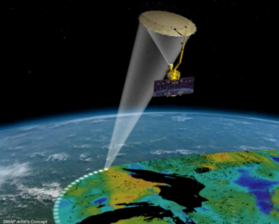
\includegraphics[width=.35\textwidth]{img/satellite.png}}\hfil
    \subfloat[Global root zone soil moisture]{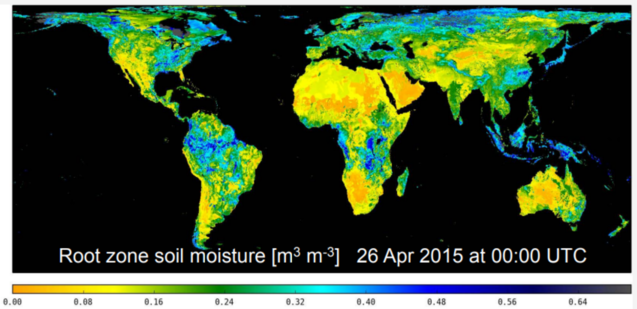
\includegraphics[width=.6\textwidth]{img/roots-global-map.png}}
    \caption{\label{fig:satellite}Examples of commercially available soil moisture sensors \cite{meter_group_teros_nodate, baseline_soil_2021, czechproject_spol_sro_pudni_2024}.}
\end{figure}

\section{\label{section:soil-moisure-sensors-theory}Capacitive soil moisture sensors}
The working principle of capacitive soil moisture sensors is based on the dielectric permittivity of the soil. Water has a high dielectric constant compared to other soil components such as air, minerals, and organic matter, as illustrated by Figure \ref{fig:dielectric-constant}. This property makes the presence of water in the soil significantly alter its dielectric permittivity.

\begin{figure}
    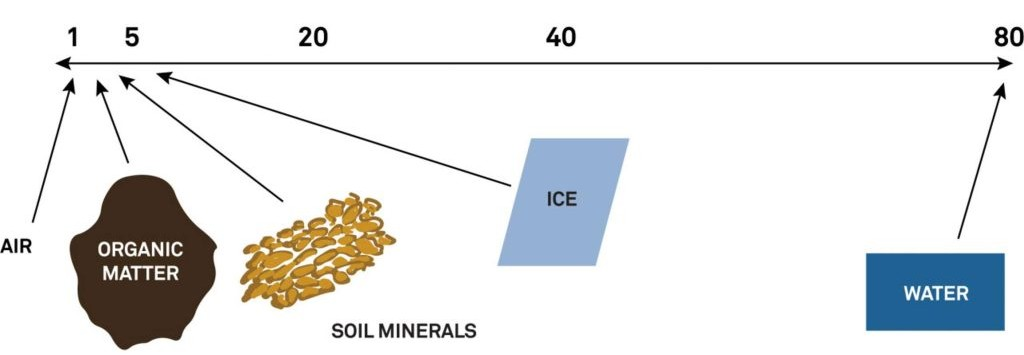
\includegraphics[width=.7\textwidth]{fig/dielectric-constant.jpg}
    \caption{\label{fig:dielectric-constant}Dielectric constant $\epsilon_r$ of various materials. Source \cite{meter_group_soil_2023}.}
\end{figure}

A typical capacitive soil moisture sensor consists of two conductive plates, which function as electrodes. These plates are separated by a non-conductive material or are directly exposed to the soil, depending on the sensor design. The plates and the soil form a capacitor. When an alternating current is applied to the electrodes, an electric field is created between them.

As the volumetric water content in the soil increases, the relative dielectric permittivity of the soil also increases due to the high dielectric constant of water. This change in permittivity affects the capacitance between the plates. Specifically, the capacitance increases as the water content rises according to the equation
\begin{equation}
    \label{equation:capacitance} C = \dfrac{\epsilon_r \epsilon_0 S}{d}
\end{equation}
where $\epsilon_0 = 8.85 \cdot 10^{-12} \frac{F}{m}$ permittivity of the vacuum, the surface area $S$ and distance between the electrodes $d$ are constant, the capacitance is proportional to the relative permittivity $\epsilon_r$.

In practice, the dielectric constant is also largely dependant on temperature, measuring frequency and saturation with dissolved ions \cite{meter_group_soil_2023,podest_applications_nodate}. This makes precise absolute measurements almost impossible without prior calibration against know reference for particular soil type.

\section{LoRa}
LoRa (Long Range) is a low-power wireless communication technology designed specifically for long-range communications with low power consumption. It is one of the leading technologies used in the rapidly expanding field of the Internet of Things (IoT), particularly in applications requiring devices to send small amounts of data over long distances while conserving battery life.

Its modulation technique is known as LoRa modulation and is derived from chirp spread spectrum (CSS) modulation. It operates in the sub-gigahertz radio frequency bands, and it is typically used in a star-of-stars network topology in conjunction with LoRaWAN (Long Range Wide Area Network), which defines the communication protocol and system architecture for the network.

LoRa is particularly noted for its excellent penetration in dense urban environments and indoor connectivity, compared to other technologies like Wi-Fi and cellular networks. This capability, combined with its low power requirements and long range, provides a distinct advantage in scenarios where alternative networking technologies might fail or be too costly.
